\documentclass[12pt, letterpaper]{article}
\title{Scrum}
\author{Agustin Salum\thanks{-}}
\date{Agosto 2023}

\usepackage{graphicx}

\begin{document}
\maketitle

    \tableofcontents % Índice general
\newpage

% Indice Agil

\section{Ágil}
Conozca el Manifiesto Ágil y cómo ha cambiado la forma en que las personas piensan sobre el desarrollo de 
software.
\index{Ágil}

% Subindice El modelo de cascada

\subsection{El modelo de cascada}
El modelo de gestion de cascada predominó en los años 80 y 90, es una metodología que se establece por 5 
caras normalmente

\vspace{10pt} % Agregar espacio de 10 puntos después de la figura

\begin{figure}[ht] % Imagen cascada
    \centering
    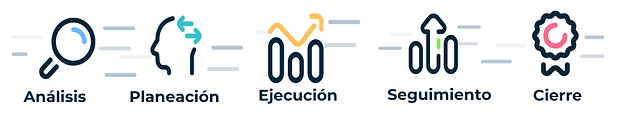
\includegraphics[width=0.8\textwidth]{imagenes/cascada.png}
    \caption{Imagen del Modelo en Cascada}
    \label{fig:cascada}
  \end{figure}

\vspace{10pt} % Agregar espacio de 10 puntos después de la figura

Una vez que se ha avanzado en cada una de estas fases del proceso ya no puedes dar marcha atrás, inpidiendo 
regresar a la fase anterior

\index{El modelo de cascada}

% Subindice El manifiesto ágil

\subsection{El manifiesto Agil}

El Manifiesto Ágil alienta a los equipos a pensar en cómo romper los silos que separan a las personas que 
trabajan en un proyecto, otorgando a las personas roles y responsabilidades formales y brindando expectativas 
de colaboración.

\vspace{10pt} % Agregar espacio de 10 puntos después de la figura

\begin{figure}[ht] % Imagen manifiesto
    \centering
    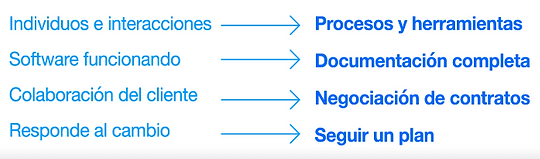
\includegraphics[width=0.8\textwidth]{imagenes/manifiesto_agil.png}
    \caption{Mientras que hay valor en los artículos de la derecha, valoramos más los artículos de la izquierda}
    \label{fig:manifiesto_agil}
  \end{figure}

\vspace{10pt} % Agregar espacio de 10 puntos después de la figura

% Título a la izquierda más pequeño que el índice y subíndice
\paragraph{Valores fundamentales del manifiesto:} El manifiesto de Agil consta de 4 valores fundamentales y 
12 principios de apoyo que lideran en enfoque ágil 
para el desarrollo de software

% Viñetas

\begin{enumerate}
    
    % Numerica
    \item Individuos e interacciones sobre procesos y herramientas
        \begin{itemize}
            % Punto
            \item Valorar a las personas más que a los procesos, ya que son las personas las que responden e 
            impulsan el proceso de desarrollo.
        \end{itemize}
    
    % Numerica
    \item Software de trabajo sobre la documentación completa
        \begin{itemize}
            % Punto
            \item Ágil no elimina la documentación, pero la simplifica de una forma que le brinda al 
            desarrollador lo que necesita para hacer el trabajo sin atascarse en los detalles.
        \end{itemize}
    
    % Numerica
    \item Colaboración del cliente sobre la negociación de contrato
        \begin{itemize}
            % Punto
            \item El manifiesto ágil describe a un cliente que está comprometido y colabora a lo largo del proceso 
            de desarrollo, esto hace que sea mucho más fácil para el desarrollo satisfacer sus necesidades del 
            cliente.
        \end{itemize}
    
    % Numerica
    \item Respondiendo al cambio sobre seguir un plan
        \begin{itemize}
            \item El desarrollo de software tradicional esperaba el cambio como un gasto, por lo que debía 
            evitarse. La intensión era desarrollar planos detallados y elaborados con un conjunto definido de 
            características y con todo generalmente teniendo una prioridad tan alta como todo lo demás y con un
             gran número de dependencias en la entrega en un cierto orden para que el equipo pueda trabajar en 
             las siguientes pieza del rompecabezas.
        \end{itemize}
\end{enumerate}

\index{El manifiesto Agil}

% Subindice Principios agiles

\subsection{Principios ágiles}

Describen una cultura en la cual el cambio es bienvenido y el trabajo se enfoca en el cliente. Consite en 
alinear el desarrollo con las habilidades comerciales.

\vspace{10pt} % Agregar espacio de 10 puntos después de la figura

\begin{figure}[ht] % Imagen principios agiles
    \centering
    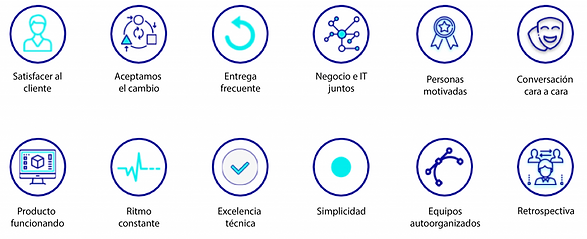
\includegraphics[width=0.8\textwidth]{imagenes/principios.png}
    \caption{Consite en alinear el desarrollo con las habilidades comerciales}
    \label{fig:principios}
  \end{figure}

\vspace{10pt} % Agregar espacio de 10 puntos después de la figura

\index{Principios ágiles}

% Indice Scrum

\section{Introduccion a Scrum}

La metodología Scrum es un modelo ágil que consiste en un marco bien definido para llevar a cabo el desarrollo 
de software en equipos.

\index{Introduccion a Scrum}

% Subindice El modelo de cascada

\subsection{Que es Scrum}

Scrum un marco de trabajo ágil en los negocios que se encaminan al futuro con innovación y tecnología.

\vspace{10pt} % Agregar espacio de 10 puntos después de la figura

\begin{figure}[ht] % Imagen scrum
    \centering
    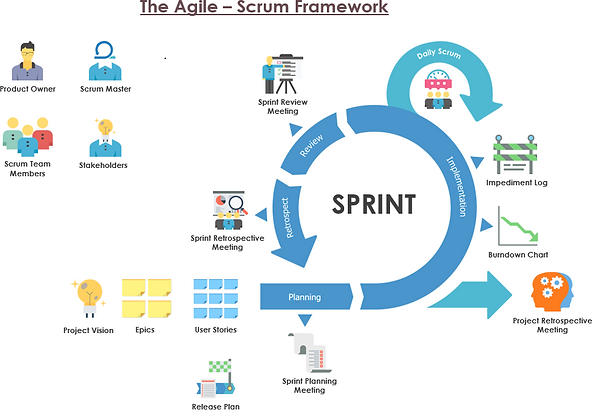
\includegraphics[width=0.6\textwidth]{imagenes/scrum.png}
    \caption{Marco de trabajo}
    \label{fig:scrum}
  \end{figure}

\vspace{10pt} % Agregar espacio de 10 puntos después de la figura

Al estar enmarcada dentro de las metodologías agile, Scrum se basa en aspectos como:
\begin{itemize}
    % Punto
    \item La \textbf{flexibilidad} en la adopción de cambios y nuevos requisitos durante un proyecto complejo.
    \item El factor \textbf{humano}.
    \item La \textbf{colaboración} e interacción con el cliente.
    \item El desarrollo iterativo como forma de asegurar buenos \textbf{resultados}.
\end{itemize}

% Título a la izquierda más pequeño que el índice y subíndice
\paragraph{Roles, Eventos y Artefactos}\textrightarrow{} A continuacion se detallan cada uno

% Viñetas

\begin{enumerate}
    
    % Numerica
    \item \textbf{Roles/responsabilidades}
        \begin{itemize}
            % Punto
            \item \underline{Product owner}
                \begin{itemize}
                    % Punto
                    \item Es responsable de definir y priorizar el backlog del producto, representando las 
                    necesidades del cliente y del negocio. Toma decisiones sobre qué características se 
                    desarrollarán y en qué orden, asegurando que el equipo desarrolle un producto de alto valor.
                    \item Es el único autorizado para manipular el Backlog.
                    \item Crea y comunica los elementos del Product Backlog.
                    \item Se asegurar de que el Product Backlog es transparente y entendido por el resto del 
                    Equipo Scrum o stakeholders.
                \end{itemize}
            
            \item \underline{Scrum master}
                \begin{itemize}
                    % Punto
                    \item Es el facilitador y líder del equipo Scrum. Su función principal es asegurar que el 
                    equipo comprenda y siga los principios y prácticas de Scrum. Elimina obstáculos y fomenta 
                    la colaboración y la mejora continua en el equipo.
                    \item Es el responsable de facilitar (implementar) el marco de trabajo SCRUM.
                    \item El Scrum Master no controla el equipo, pero trabaja para remover cualquier obstáculo 
                    que les impida lograr los objetivos del sprint.
                    \item Dar servicio al Product Owner: ayudando a encontrar técnicas para la definición del 
                    Product Goal y efectiva gestión del Product Backlog.
                \end{itemize}

            \item \underline{Developer}
                \begin{itemize}
                    % Punto
                    \item Es el grupo de profesionales encargados de llevar a cabo el trabajo para entregar el 
                    incremento del producto. Son autónomos y se organizan internamente para realizar el trabajo 
                    de manera eficiente.
                    \item Crea el Sprint Backlog.
                    \item Adapta el Sprint Backlog a diario, valorando el progreso hacia la consecución del 
                    Sprint Goal.
                \end{itemize}

            \item \underline{Stakeholders}
                \begin{itemize}
                    % Punto
                    \item Son las personas o grupos interesados en el producto y que tienen algún tipo de 
                    influencia o interés en su desarrollo y éxito. Los stakeholders brindan retroalimentación y 
                    pueden participar en las revisiones de Sprint para verificar el progreso del equipo.
                \end{itemize}

        \end{itemize}

    % Numerica
    \item \textbf{Eventos}
        \begin{itemize}
            % Punto
            \item \underline{Sprint Planning}
                \begin{itemize}
                    % Punto
                    \item Es una reunión al comienzo de cada sprint, donde el equipo Scrum y el Product Owner 
                    definen las metas y el alcance del sprint. Se seleccionan las tareas a abordar y se 
                    establece el plan para el incremento del producto.
                    \item
                \end{itemize}

            \item \underline{Daily Scrum}
                \begin{itemize}
                    % Punto
                    \item Es una breve reunión diaria de 15 minutos, donde el equipo de desarrollo sincroniza 
                    su trabajo. Cada miembro del equipo comparte qué hizo el día anterior, qué planea hacer hoy 
                    y si hay obstáculos que necesiten ser abordados.
                \end{itemize}

            \item \underline{Sprint review}
                \begin{itemize}
                    % Punto
                    \item Es una reunión al final de cada sprint, donde el equipo presenta el incremento del 
                    producto completado al Product Owner y otros stakeholders. Se obtiene retroalimentación y 
                    se revisan las metas cumplidas.
                \end{itemize}

            \item \underline{Sprint retrospective}
                \begin{itemize}
                    % Punto
                    \item Es una reunión que se lleva a cabo después del Sprint Review, donde el equipo Scrum 
                    reflexiona sobre el sprint que acaba de terminar. Identifican qué funcionó bien, qué puede 
                    mejorarse y definen acciones para implementar mejoras en el siguiente sprint.
                \end{itemize}

            \item \underline{Sprint refinement}
                \begin{itemize}
                    % Punto
                    \item Aunque no es un evento formal en el Scrum Guide, es una práctica común. En este 
                    evento, el equipo revisa y actualiza el backlog del producto, añade detalles a las 
                    historias de usuario y las prioriza para futuros sprints. Es una oportunidad para 
                    preparar las próximas tareas a medida que se acerca el siguiente Sprint Planning.
                \end{itemize}

        \end{itemize}
    
    % Numerica
    \item \textbf{Artefactos}
        \begin{itemize}
            % Punto
            \item \underline{Product Backlog}
                \begin{itemize}
                    % Punto
                    \item Es una lista ordenada de todas las funcionalidades, características, mejoras y 
                    correcciones que se desean para el producto. Es responsabilidad del Product Owner 
                    mantenerlo actualizado, priorizar los elementos y asegurarse de que estén claros y listos 
                    para ser implementados por el equipo.
                \end{itemize}

            \item \underline{Sprint Backlog}
                \begin{itemize}
                    % Punto
                    \item Es una lista de las tareas específicas seleccionadas del Product Backlog para el 
                    sprint actual. El equipo de desarrollo decide qué elementos del Product Backlog se 
                    abordarán durante el sprint y descompone esos elementos en tareas más pequeñas. Es una 
                    planificación detallada para el trabajo del sprint.
                \end{itemize}

            \item \underline{Increment}
                \begin{itemize}
                    % Punto
                    \item Es el resultado tangible del trabajo realizado durante un sprint. Es el producto 
                    con todas las funcionalidades y mejoras completadas durante el sprint, más cualquier 
                    trabajo adicional realizado para asegurar la calidad del producto. Al final de cada 
                    sprint, el incremento debe ser potencialmente entregable y listo para ser liberado.
                \end{itemize}

        \end{itemize}
    
\end{enumerate}

\index{Que es Scrum}

% Subindice Que es Sprint

\subsection{Qué es Sprint}

El Sprint es la unidad básica de trabajo para un equipo Scrum, y puede ser la característica de Scrum que más 
lo diferencia de otros modelos Agile. Un sprint es una sola iteración llevada a cabo por un equipo.

Sprint es un contenedor para el resto de eventos de Scrum. El Sprint es continuo, es decir , su duración no 
debe cambiar mientras está en marcha el desarrollo del producto , y se puede interpretar como una medida de 
ritmo constante a lo largo del tiempo.

\index{Qué es Sprint}

\end{document}